%
\documentclass[12pt]{article}

%% make references and citations clickable
%\usepackage[backref,colorlinks=true, linkcolor=blue, citecolor=blue, urlcolor=blue, pdfborder={0 0 0}]{hyperref}

%% set the paper geometry
\usepackage[left=1in,top=1in,right=1in,bottom=1in,letterpaper]{geometry}

%% this is for arrows with text over them
\usepackage{mathtools}

%% uncomment the next line if you need to present an algorithm
%\usepackage{algorithm,algorithmic}

% This section is added by me (Geoff)
%-----------------------------------------------
%% standard AMS stuff
\usepackage{amssymb,amsmath}

%% some proof-writing environments
\newenvironment{claim}[1]{\par\noindent\underline{Claim:}\space#1}{}
\newenvironment{claimproof}[1]{\par\noindent\underline{Proof:}\space#1}{}

%% norm and abs val and inner prod
\newcommand{\norm}[1]{\left\lVert#1\right\rVert}
\newcommand{\abs}[1]{\left\lvert#1\right\rvert}
\newcommand{\iprod}[2]{\langle#1 , #2 \rangle}
\newcommand{\spn}[0]{\text{span}}

%% ceiling and floor
\DeclarePairedDelimiter\ceil{\lceil}{\rceil}
\DeclarePairedDelimiter\floor{\lfloor}{\rfloor}

%% kernel and image  -- Currently did something wrong
%%\newcommand{\ker}[1]{\text{ker}\left(#1\right)}
%%\newcommand{\Im}[1]{\text{Im}\left(#1\right)}  %% TODO: FIX THIS

%% Important letters/symbols
\newcommand{\ep}[0]{\epsilon}
\newcommand{\R}[0]{\mathbb{R}}

%% I had some issues with alignment, here was one online soln
%%\usepackage[fleqn]{amsmath}
%% It DIDN'T WORK THOUGH

% very specific stuff
\iffalse
\newcommand{\bt}{\boldsymbol{\times}}

%% stability and floating point stuff
\newcommand{\fl}[1]{\text{fl}\left(#1\right)}
\newcommand{\epm}[0]{\epsilon_{mach}}
\fi

%% standard theorem environments
\newtheorem{theorem}{Theorem}[section]
\newtheorem{lemma}[theorem]{Lemma}
\newtheorem{proposition}[theorem]{Proposition}
\newtheorem{corollary}[theorem]{Corollary}

%------------------------------------------------


%% for including urls by \url{url text}
\usepackage{url}

\begin{document} 

\title{Hyperspectral Imaging}
\author{Geoffrey Iyer}
\maketitle
%\begin{abstract}
%Here is an abstract
%\end{abstract}
\tableofcontents

\section{Introduction}

A relatively recent development in remote sensing technology is the creation of hyperspectral cameras. Whereas the human eye primarily sees color in three wavelenghts (red, green, blue), a hyperspectral sensor collects data from a much larger range of the spectrum. Each wavelength collected is called a ``band'', and most hyperspectral sensors sample 100-200 bands, ranging from microwaves to UV rays. This data can be used to differentiate objects that would appear the same to a standard camera.

In this project we aim to perform unsupervised classification on hyperspectral images using a spectral clustering algorithm. This requires defining the Graph Laplacian matrix associated to our data (Section \ref{sec:GraphLaplacian}) and computing eigenvectors and eigenvalues of the matrix (Section \ref{sec:SpectralClustering}). In Section \ref{sec:results} we show an application of our algorithm to a sample data set.

\section{Graph Laplacian} \label{sec:GraphLaplacian}
We approach this problem via graph-based methods. A more detailed survey of the theory can be found in \cite{ref:SpectralClustering2}. Here we state only the results necessary to implement our algorithm.

\subsection{Similarity Graphs}
We can represent a hyperspectral image using an undirected graph $G = (V,E)$. The nodes $v_i\in V$ of the graph correspond to the pixels in the image. We give each edge $e_{ij}$ a \emph{weight} $w_{ij}\geq 0$ representing the similarity between nodes $v_i, v_j$. This gives rise to a \emph{similarity matrix} (also called the \emph{weight matrix}) \[W = \left(w_{ij}\right)_{i,j=1}^n.\] Since $G$ is undirected, we require that $w_{ij} = w_{ji}$, which implies that $W$ is a symmetric matrix. There are several popular means to measure ``similarity'' between nodes, which we shall discuss in more detail in \ref{EdgeWeights}.

\subsection{Graph Min-Cut Problem} \label{GraphMinCut}
The problem of unsupervised clustering can be rephrased as a graph-cut-minimization problem of the similarity matrix $W$. Given a set $A\subseteq V$, we define the \emph{graph-cut} \[cut(A,A^c) = \frac{1}{2}\sum_{v_i \in A, v_j \in A^c} w_{ij}.\] Or, more generally, for disjoint sets $A_1, A_2, \ldots, A_k$ such that $\cup_{j=1}^kA_j = V$ we define \[cut(A_1,\ldots,A_k) = \frac{1}{2}\sum_{v_{i} \in A_m, v_j \notin A_m}w_{ij}.\]

Each choice of sets $A_1,\ldots,A_k$ partitions our image into $k$ classes. Finding an optimal $A_1,\ldots,A_k$ corresponds to minimizing the energy in the graph cut.

\subsection{Definition of Graph Laplacian}

Once we have formed the weight matrix $W$, we can use it to define the Graph Laplacian. For each node $v_i\in V$, define the \emph{degree} of the node \[d_i = \sum_j w_{ij}.\] Intuitively, the degree represents the strength of a node. Let $D$ be the diagonal matrix with $d_i$ as the $i$-th diagonal entry. We then define the \emph{unnormalized Graph Laplacian} \[L = D - W,\] and the \emph{normalized Graph Laplacian} \[L_{sym} = D^{-1/2}LD^{-1/2} = I - D^{-1/2}WD^{-1/2}.\] For a thorough explanation of the properties of the Graph Laplacian, see \cite{ref:GraphLaplacian1}. In our algorithm we will use the following properties.

\begin{theorem}
\begin{itemize}
\item For every $f\in\mathbb{R}^n$ we have \[f^TLf = \frac{1}{2}\sum_{i,j=1}^nw_{ij}(f_i-f_j)^2\]
\[f^TL_{sym}f = \frac{1}{2}\sum_{i,j=1}^n w_{ij}\left(\frac{f_i}{\sqrt{d_i}}-\frac{f_j}{\sqrt{d_j}}\right)^2\] \label{GLiprod}
\item $L, L_{sym}$ are both symmetric and positive semidefinite
\item The eigenvectors of $L$ (or $L_{sym}$) corresponding to eigenvalues of small magnitude give an approximate solution to the graph min-cut problem posed in \ref{GraphMinCut}.
\end{itemize}
\end{theorem}


%%%%%%%%%%%%%%%%%%%%%%%%%%%%%%%%
%%% I want to cut this material
%%%%%%%%%%%%%%%%%%%%%%%%%%%%%%%%

% We use the Graph Laplacian to solve the min-cut problem posed in \ref{GraphMinCut}. For let $f:V\to \{-1,1\}$, and define $A=f^{-1}(1)$. Then by theorem \ref{GLiprod} we have
% \begin{align*}
% f^TLf &= \frac{1}{2}\sum_{i,j=1}^nw_{ij}(f_i-f_j)^2 \\
% &= \frac{1}{2}\sum_{v_i\in A, v_j\in A^c}w_{ij} \\
% &= cut(A,A^c) \\
% \end{align*}

% Solving the graph min-cut problem is equivalent to finding $f:V\to \{-1,1\}$ minimizing $f^TLf$. Unfortunately, solving this problem is $O(\abs{V}^{4})$. More generally, to partition $V$ into $k$ classes is $O(\abs{V}^{k^2})$ \cite{ref:GraphMinCut}. Instead we solve the relaxed problem \[\min_{f\in\mathbb{R}^n}\sum w_{ij}(f_i-f_j)^2\] via finding eigenvectors of $L$.


% Similarly, can find \[\min_{f\in\mathbb{R}^n} \sum w_{ij}\left(\frac{f_i}{\sqrt{d_i}}-\frac{f_j}{\sqrt{d_j}}\right)^2\] via eigenvectors of $L_{sym}$.
% \\~\\
% Project $f$ into $\{-1,1\}^n$ to get an approximate graph min cut

%%%%%%%%%%%%%%%%%%%%%%
%%% End cut
%%%%%%%%%%%%%%%%%%%%%%

\subsection{Edge Weights and Sparsification}\label{EdgeWeights}

For $v_i,v_j\in V$, we define the weight of the edge $e_{ij}$ via \[w_{ij} = \text{exp}(\norm{v_i - v_j}/\tau).\] Here $\tau$ is a scaling parameter, and $\norm{\cdot}$ can be any method of measuring distance between nodes. In this project we considered both the Euclidean norm as well as the vector angle norm for our distance measure. Intuitively the vector angle norm (aka cosine similarity, aka angular distance) seems more relevant when working with hyperspectral data.
\begin{align*}
\norm{v_i - v_j} &= \cos^{-1}\left(\frac{\iprod{x_i}{x_j}}{\norm{x_i}\cdot\norm{x_j}}\right). \\
&= \text{angle between $x_i,x_j$}\\
\end{align*}
This method ignores amplitude of a wave and focuses on shape, as can be seen in the example classification in Figures \ref{fig:StripeOriginal}, \ref{fig:StripeEuclidean}, \ref{fig:StripeVectorAngle}. However, when working with actual image we noticed very little difference between the two norms.

\begin{figure}
\begin{minipage}{.45\textwidth}
  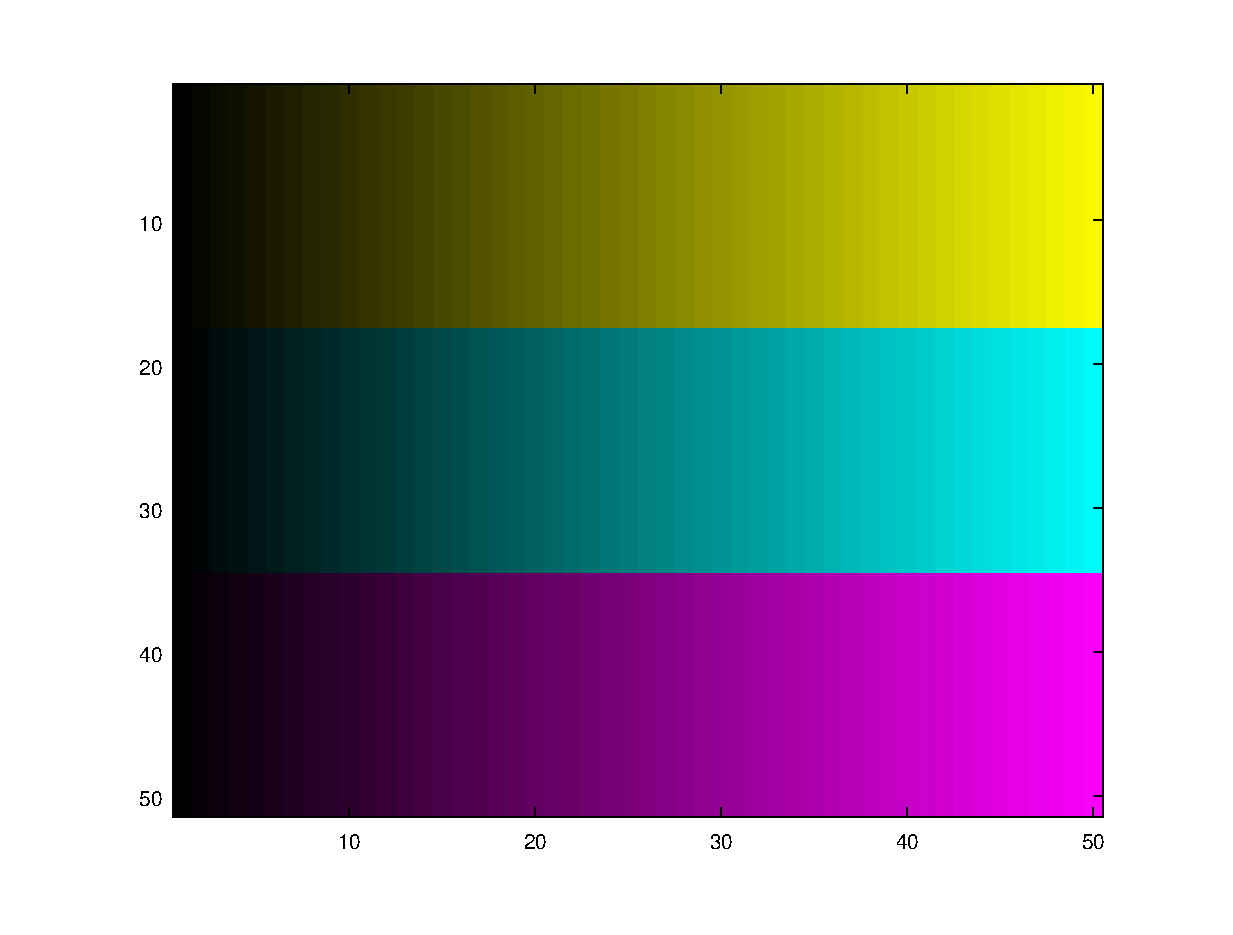
\includegraphics[width=\linewidth]{./Images/simpleStripes/image.eps}
  \caption{Original Image}
  \label{fig:StripeOriginal}
\end{minipage}\hfill
\begin{minipage}{.45\textwidth}
  \includegraphics[width=\linewidth]{./Images/simpleStripes/badClassify.eps}
  \caption{Classified with Euclidean Norm}
  \label{fig:StripeEuclidean}
\end{minipage}
\end{figure}
\begin{figure}
  \centering
  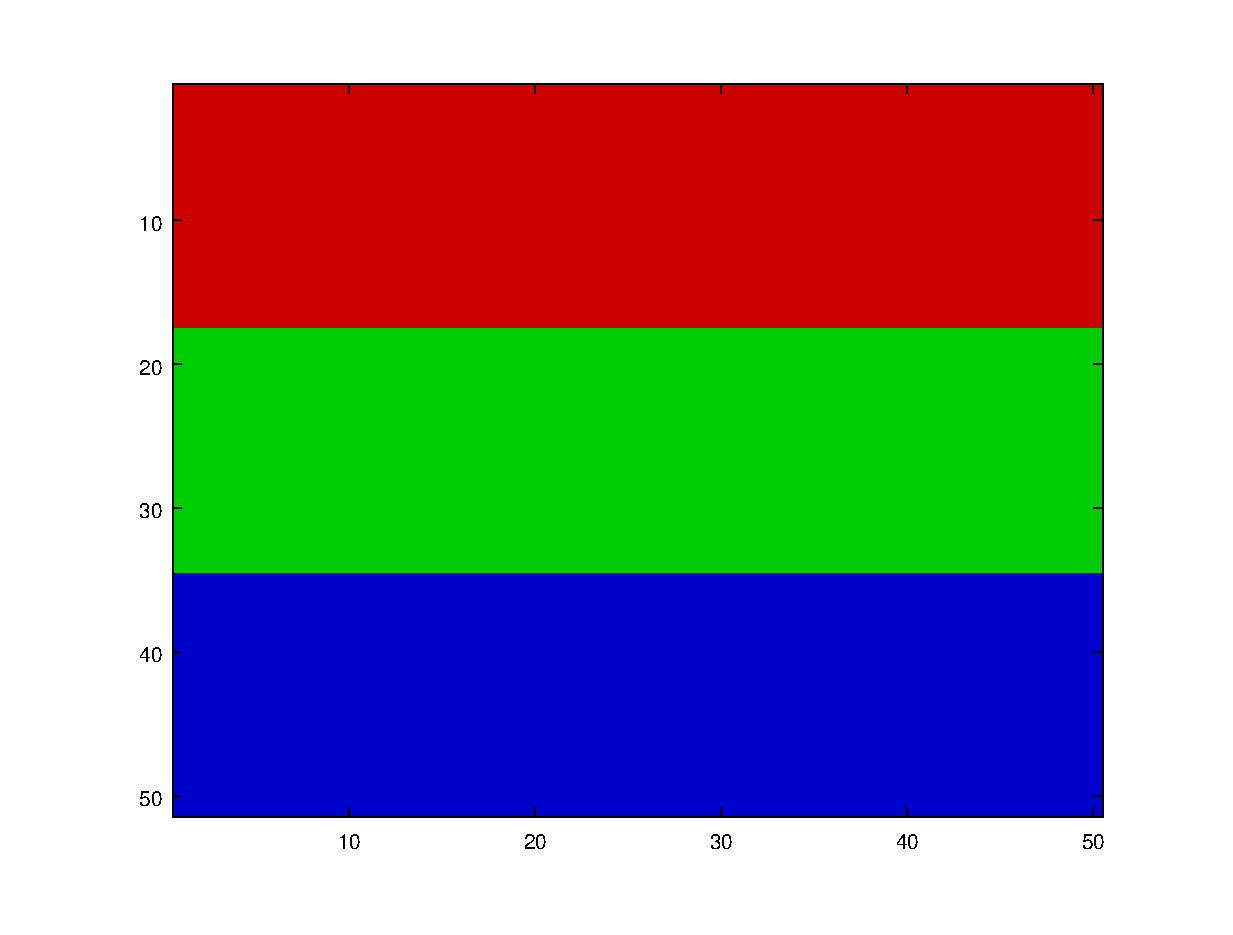
\includegraphics[width=.45\linewidth]{./Images/simpleStripes/classify.eps}
  \caption{Classified with Vector Angle}
  \label{fig:StripeVectorAngle}
\end{figure}

Using the method above will result in a dense Graph Laplacian matrix $L$, which is undesirable for finding eigenvalues and eigenvectors. Therefore we sparsify the matrix by thresholding relatively small weights to 0.

%%%%%%%%%%%%%%%%%%%%%%%%%%%%%%%%%%%%%%%%%
%% Planning to cut stuff about sparsify
%%%%%%%%%%%%%%%%%%%%%%%%%%%%%%%%%%%%%%%%%

% To help us actually compute eigenvectors/eigenvalues, we want to sparsify the Graph Laplacian matrix.
% \\~\\
% One idea we had: only compute distance of nearby pixels.
% \begin{itemize}
% \item More specifically: Only compare pixels that are close together on the physical image.
% \item Ex: Bottom-left corner and top-right corner are never compared. Considered infinitely far apart.
% \end{itemize}
% Turns out this was a bad idea. It should work well if groups are very clustered, but that was not the case for any of our datasets.
% \begin{figure}
% \begin{minipage}{.45\textwidth}
%   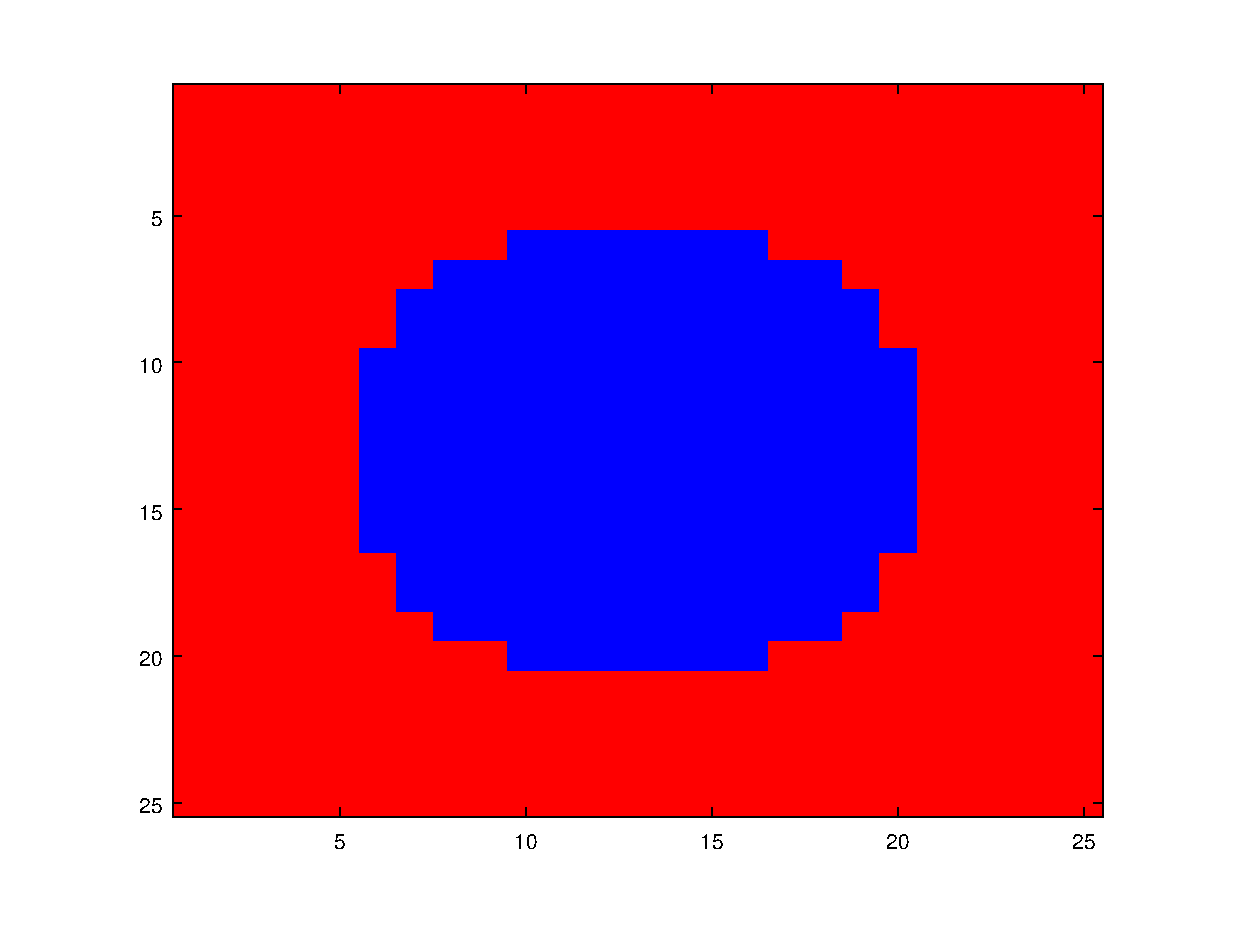
\includegraphics[width=\linewidth]{./Images/circle/image.eps}
%   \caption{Original Image}
% \end{minipage}\hfill
% \begin{minipage}{.45\textwidth}
%   \includegraphics[width=\linewidth]{./Images/circle/badClassify.eps}
%   \caption{Classified Image}
% \end{minipage}
% \end{figure}
% I wound up using basic thresholding. Pick a tolerance $tol$. If $\norm{x_i-x_j}>tol$ then $w_{ij}=0$.
% \begin{figure}
% \begin{minipage}{.45\textwidth}
%   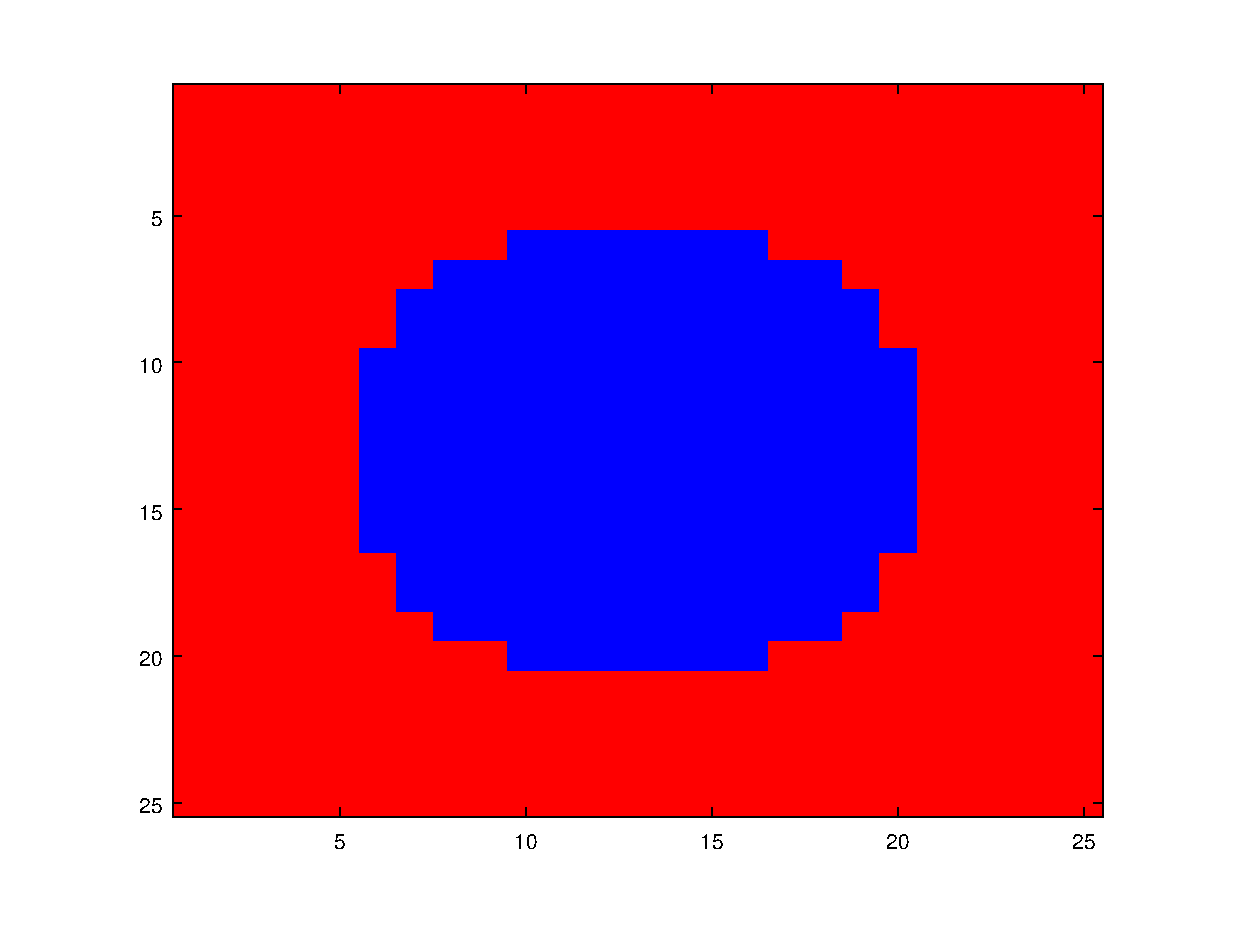
\includegraphics[width=\linewidth]{./Images/circle/image.eps}
%   \caption{Original Image}
% \end{minipage}\hfill
% \begin{minipage}{.45\textwidth}
%   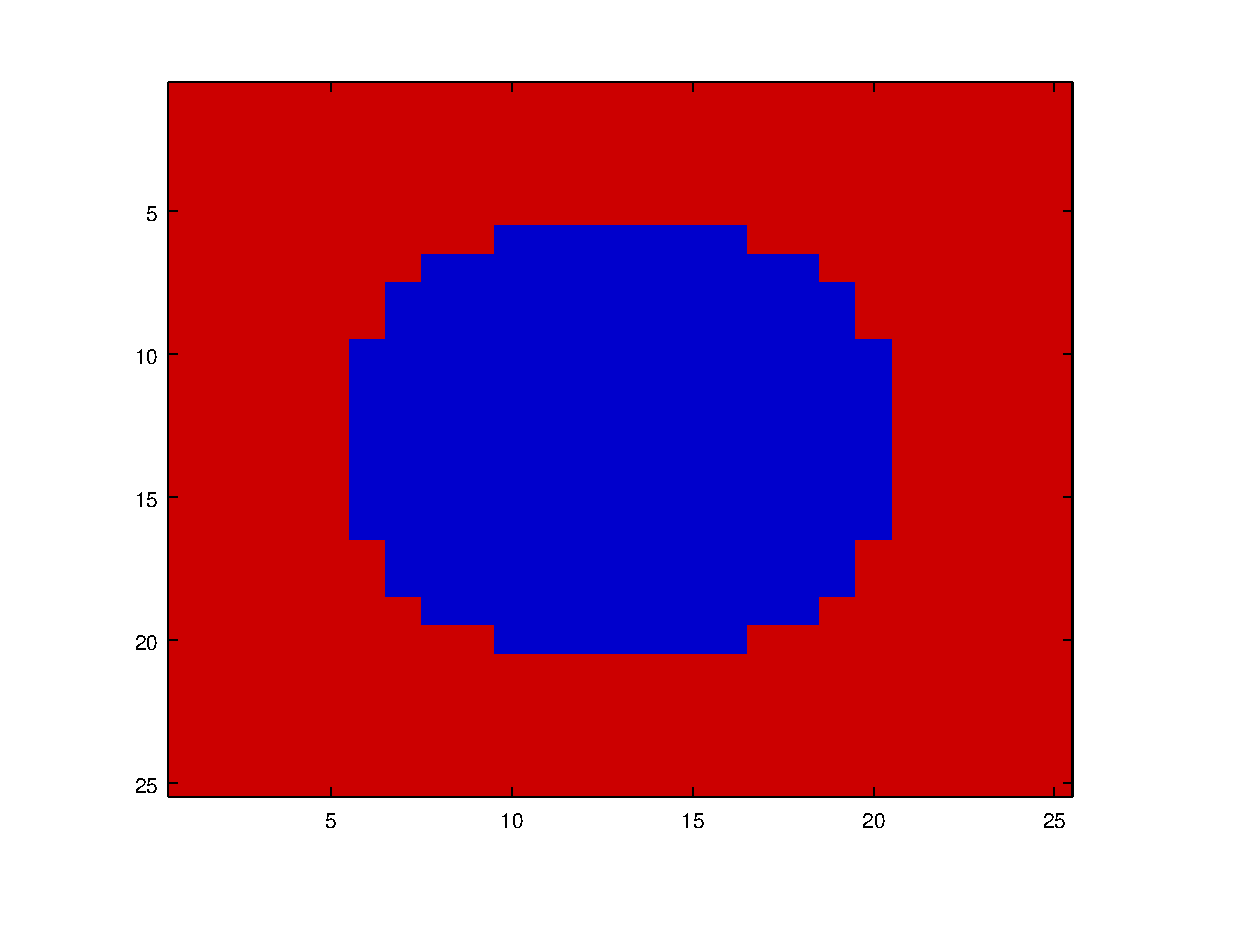
\includegraphics[width=\linewidth]{./Images/circle/classify.eps}
%   \caption{Classified Image}
% \end{minipage}
% \end{figure}
% Disadvantage: Need to look at each pair of pixels. $\approx n^2$ operations (where $n = $ number of pixels).

%%%%%%%%%%%%%%%%%%%%%%%%%%%%
%% End cuts
%%%%%%%%%%%%%%%%%%%%%%%%%%%%

\section{Spectral Clustering} \label{sec:SpectralClustering}
Having created a Graph Laplacian matrix, we apply a spectral clustering algorithm from \cite{ref:SpectralClustering1} to separate our data into classes.

Have $0\leq\lambda_1\leq\lambda_2\leq\cdots\leq\lambda_m$ the smallest $m$ eigenvalues of $L$. $f_1,\ldots,f_m$ the corresponding eigenvectors. For each pixel $v_i$ we get a vector $y_i\in\mathbb{R}^m$ given by $y_i = ((f_1)_i,\ldots,(f_m)_i)$. Run $k$-means on the $y_i$ to cluster the pixels $v_i$ into classes $C_1,C_2,\ldots,C_k$.

\subsection{Rayleigh-Chebyshev}
To find the required eigenvectors and eigenvalues for spectral clustering we use the Rayleigh-Chebyshev method developed by Chris Anderson, explained in \cite{ref:RayleighChebyshev}. A simplified version of the algorithm is given below:

\begin{itemize}
\item If $\lambda$ is an eigenvalue of $A$, and $p$ is a polynomial, then $p(\lambda)$ an eval of $p(A)$.
\item Pick $p$ such that $p(\lambda)$ is large for $\lambda$ near zero, and $p(\lambda)$ is small for $\lambda$ far from zero.
\begin{itemize}
\item Chebyshev polynomials have this property, hence the name of the algorithm.
\end{itemize}
\item Apply the power method to $p(A)$ to find the eigenvectors corresponding to \[\{\text{eigenvalues }\lambda ~ \vert ~ \abs{\lambda} \text{ relatively small}\}.\]
\end{itemize}

\section{Application to Pavia University Dataset}\label{sec:results}

To test our algorithm, we use the a scene of Pavia University, Pavia, Italy\cite{ref:Pavia} taken by the ROSIS sensor\cite{ref:ROSISsensor}. The image is $610\times340$ pixels, where each pixel represents roughly $1.3m^2$ of surface area. For each pixel, 103 different wavelengths are captured, covering values of the electromagnetic spectrum from microwaves to UV. Figures \ref{PaviaLow}, \ref{PaviaHigh}, are example bands chosen from the full 103. They are placed alongside a grayscale image of the university (Figure \ref{PaviaGray}) for easy comparison. 

This dataset also comes with a hand-labeled ``ground truth'' (Figure \ref{PaviaGroundTruth}, Table \ref{table:PaviaGroundTruth}) which we will compare against our clustering results. The ground truth divides the image into 9 classes. 

\begin{table}
\centering
\label{table:PaviaGroundTruth}
\begin{tabular}{l l l}
\textbf{\#} & \textbf{Class} & \textbf{Samples}\\
1 & Asphalt & 6631 \\
2 & Meadows & 18649 \\
3 & Gravel & 2099 \\
4 & Trees & 3064 \\ 
5 & Painted metal sheets & 1345 \\
6 & Bare Soil & 5029 \\
7 & Bitumen & 1330 \\
8 & Self-Blocking Bricks & 3682 \\
9 & Shadows & 947 \\
\end{tabular}
\caption{9 Classes of Pixel}
\end{table}

\begin{figure}
\begin{minipage}{.45\textwidth}
  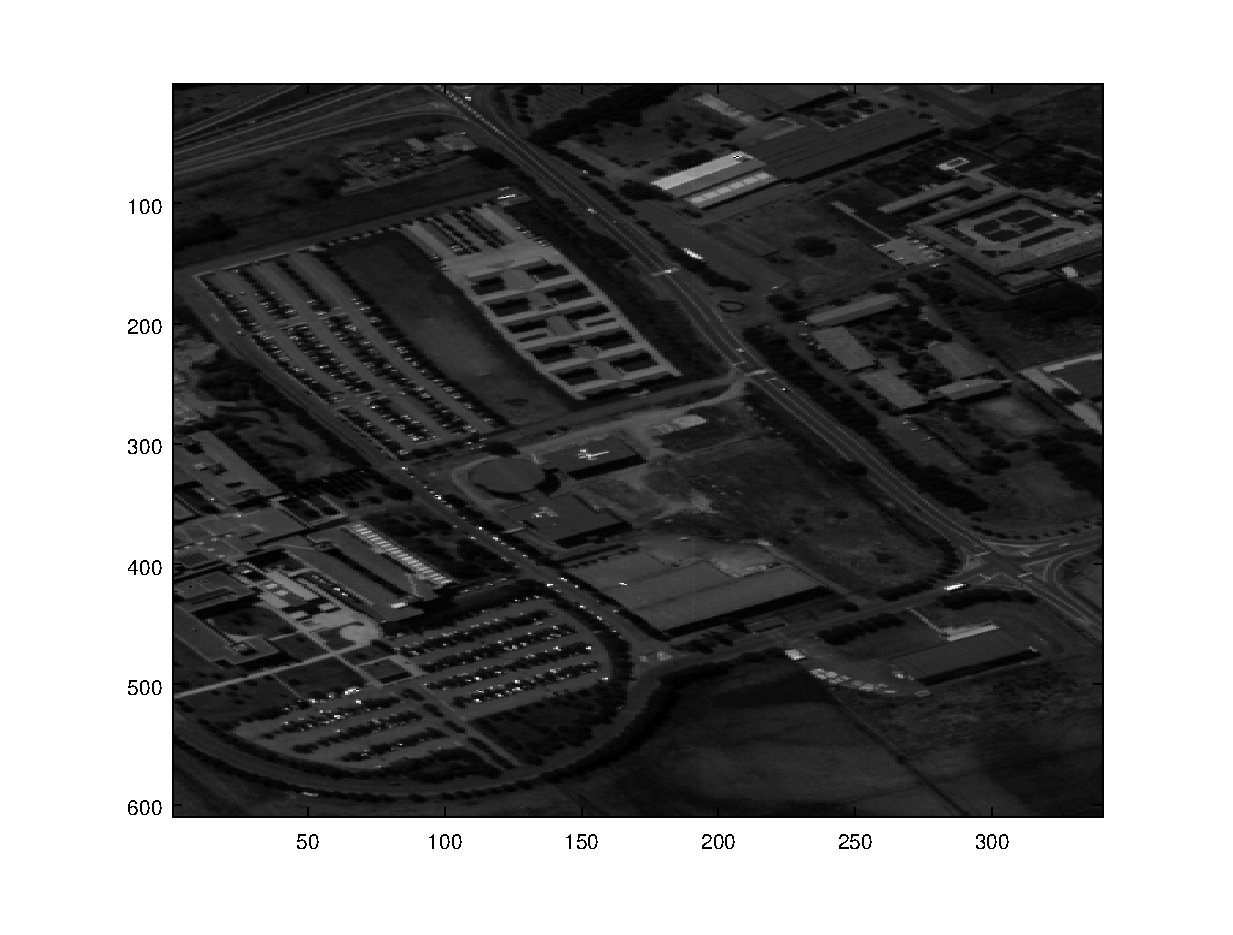
\includegraphics[width=\linewidth]{./Images/paviaFull/gray.eps}
  \caption{Grayscale Image}
  \label{PaviaGray}
\end{minipage}\hfill
\begin{minipage}{.45\textwidth}
  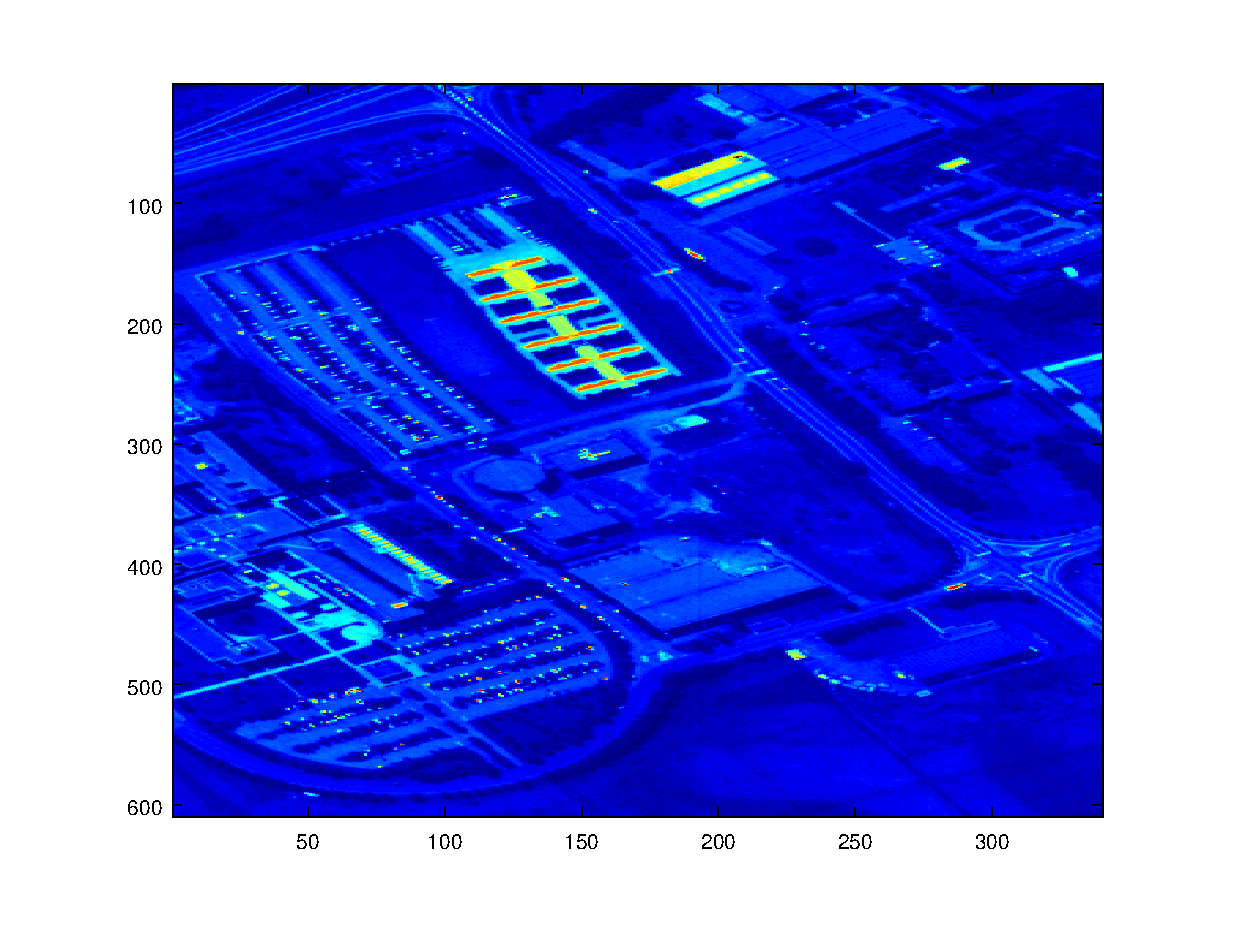
\includegraphics[width=\linewidth]{./Images/paviaFull/band21.eps}
  \caption{Low Wavelength}
  \label{PaviaLow}
\end{minipage}
\end{figure}

\begin{figure}
\begin{minipage}{.45\textwidth}
  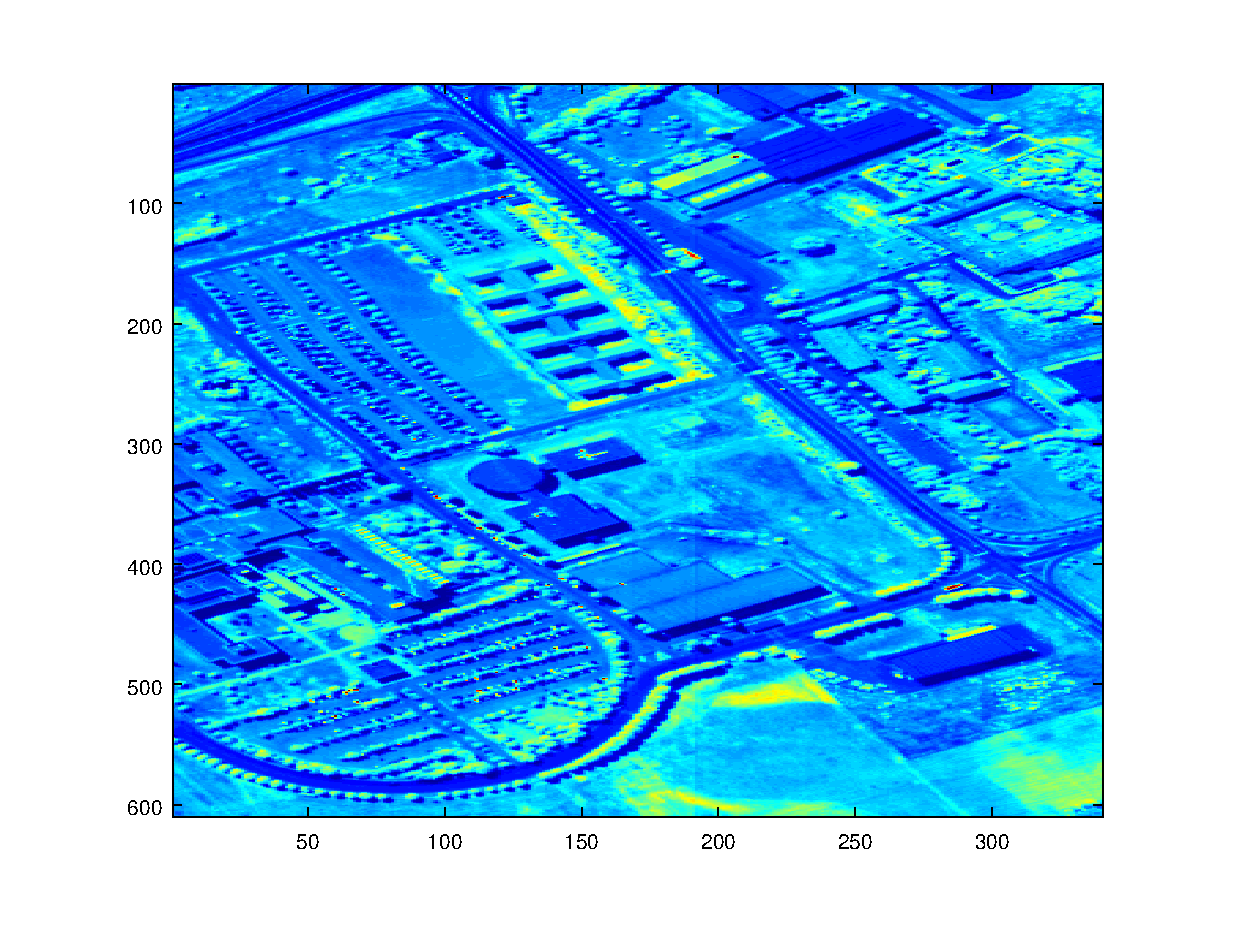
\includegraphics[width=\linewidth]{./Images/paviaFull/band81.eps}
  \caption{High Wavelength}
  \label{PaviaHigh}
\end{minipage}\hfill
\begin{minipage}{.45\textwidth}
  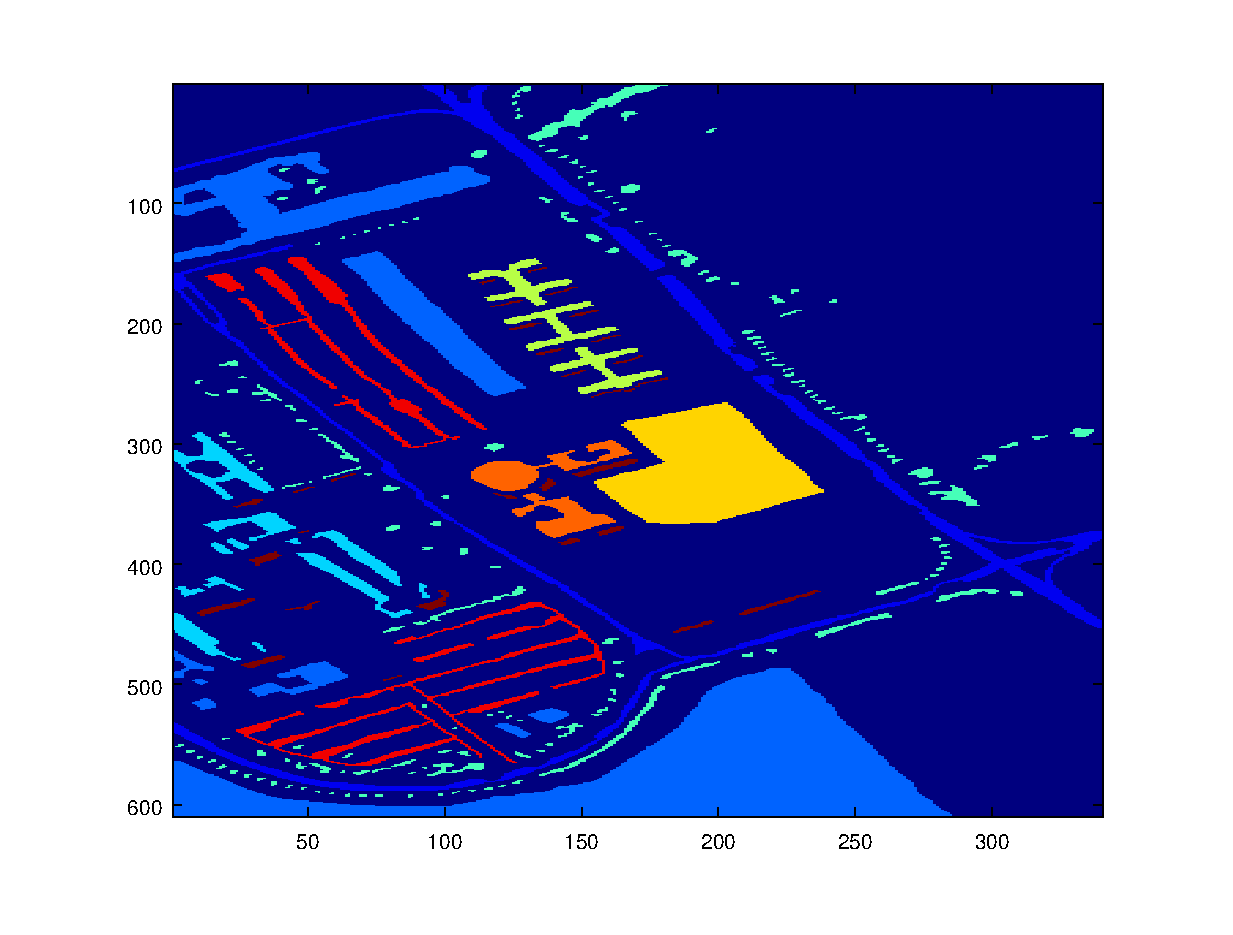
\includegraphics[width=\linewidth]{./Images/paviaFull/groundtruth.eps}
  \caption{Ground Truth}
  \label{PaviaGroundTruth}
\end{minipage}
\end{figure}

Unfortunately, our algorithm was not efficient enough to classify the entire Pavia University image, so instead we restrict our attention to a $100\times 100$ sub-picture.

\subsection{Sub-Picture}

To test our clustering algorithm, we chose a section near the center of the image that contains a building, surrounded by a meadow. Figures \ref{fig:PaviaSubGray}, \ref{fig:PaviaSubMid}, \ref{fig:PaviaSubResult}, \ref{fig:PaviaSubGroundTruth} show a grayscale image, a selected band, the spectral clustering result, and the ground truth (respectively). Comparing the clustering result against the ground truth, we get that this method correctly matched 54.7\% of pixels.

\begin{figure}
\begin{minipage}{.5\textwidth}
  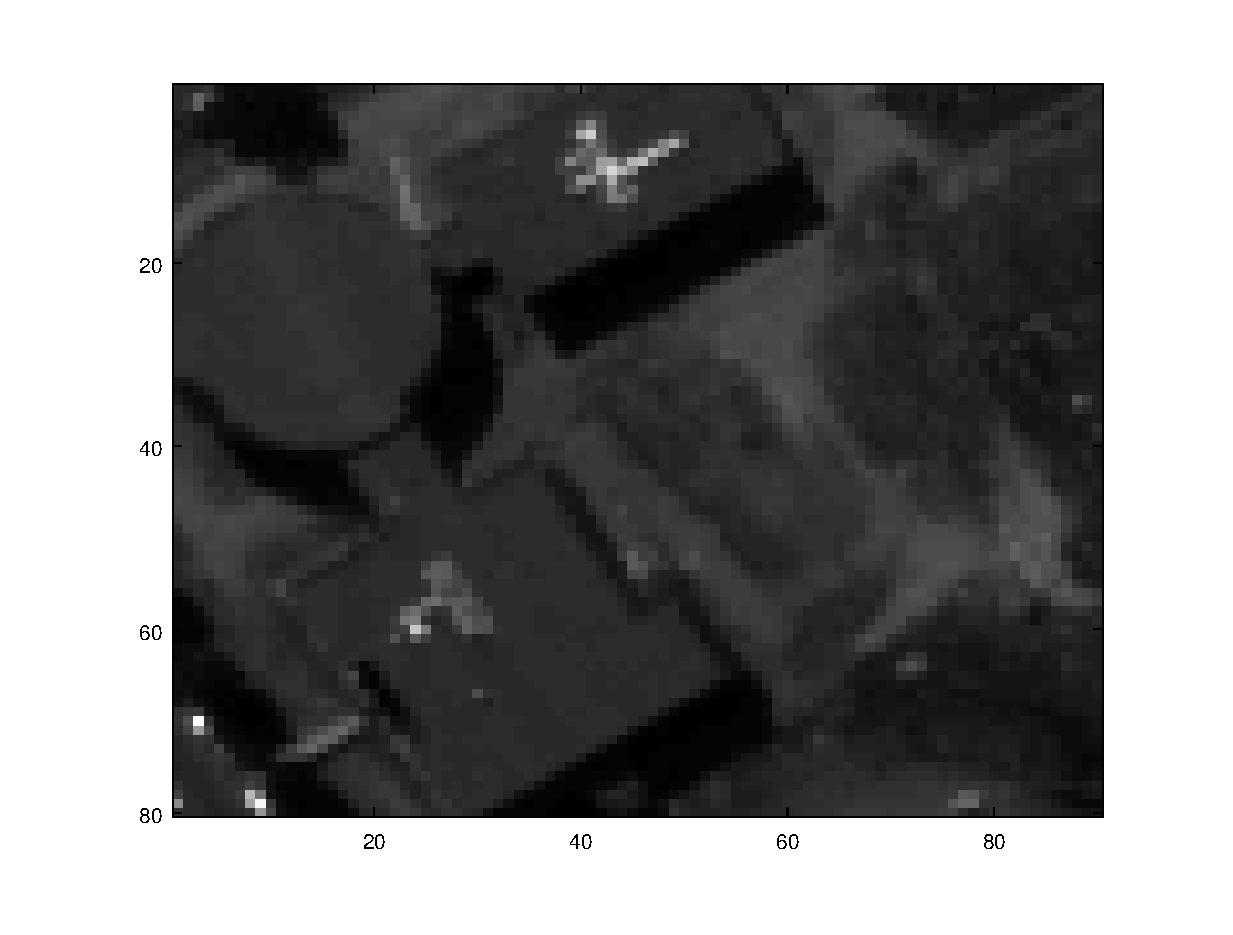
\includegraphics[width=\linewidth]{./Images/paviaSub/gray.eps}
  \caption{Grayscale Image}
  \label{fig:PaviaSubGray}
\end{minipage}\hfill
\begin{minipage}{.5\textwidth}
  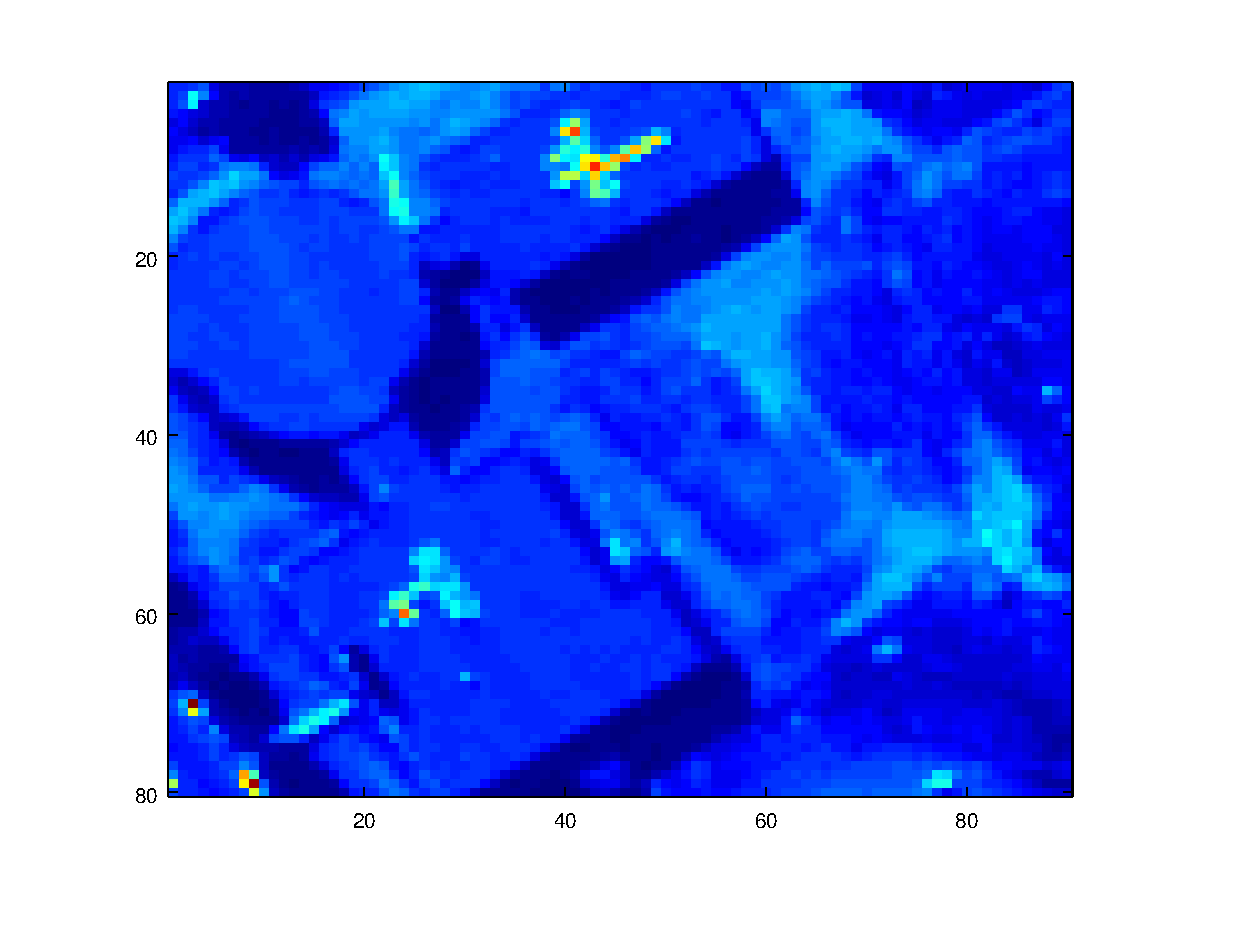
\includegraphics[width=\linewidth]{./Images/paviaSub/band51.eps}
  \caption{Mid Wavelength}
  \label{fig:PaviaSubMid}
\end{minipage}
\end{figure}
\begin{figure}
\begin{minipage}{.5\textwidth}
  \includegraphics[width=\linewidth]{./Images/paviaSub/myresult.eps}
  \caption{Spectral Clustering Result}
  \label{fig:PaviaSubResult}
\end{minipage}\hfill
\begin{minipage}{.5\textwidth}
  \includegraphics[width=\linewidth]{./Images/paviaSub/groundtruth.eps}
  \caption{Ground Truth}
  \label{fig:PaviaSubGroundTruth}
\end{minipage}
\end{figure}
% Here is another subset of the full Pavia University image.
% \begin{figure}
% \begin{minipage}{.5\textwidth}
%   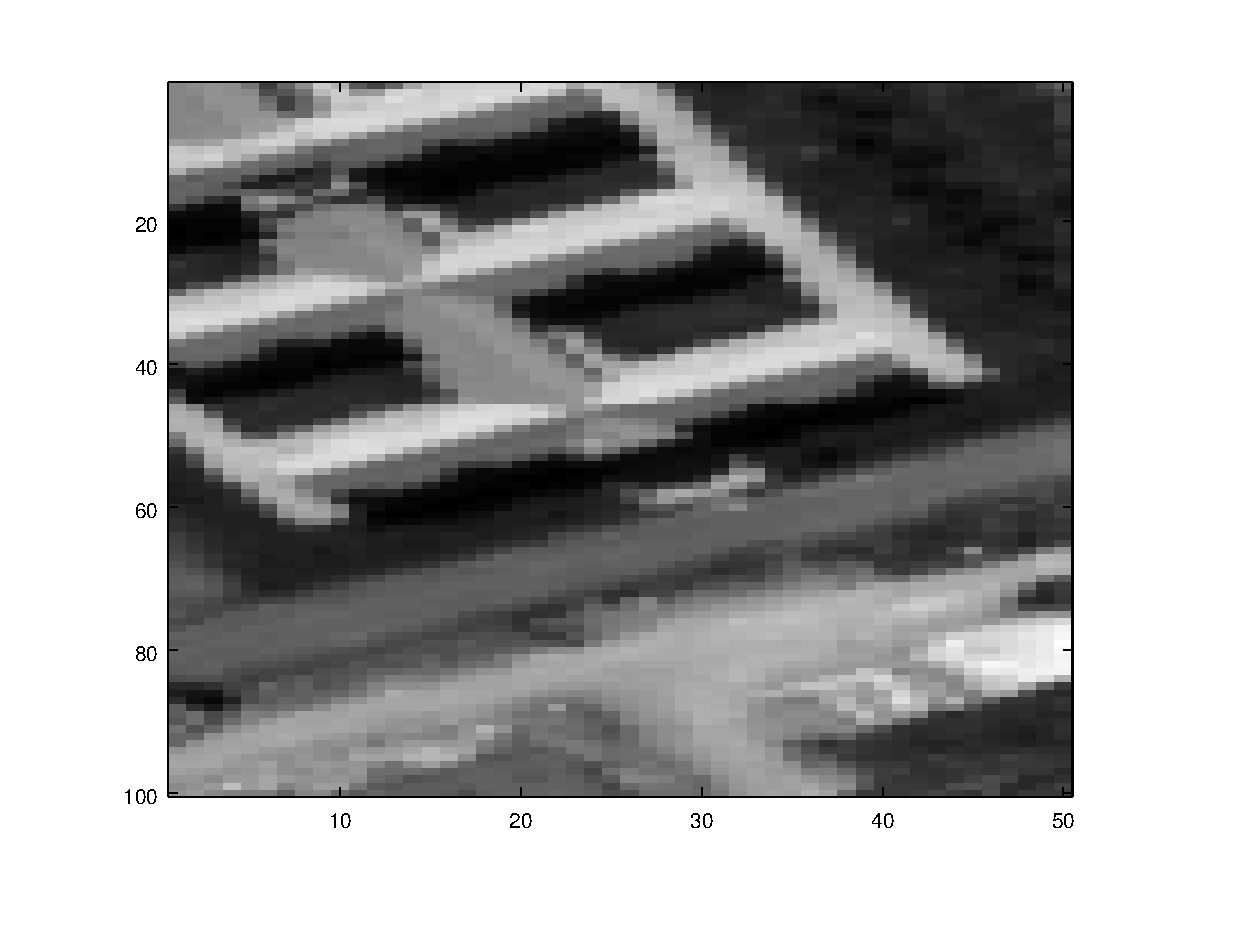
\includegraphics[width=\linewidth]{./Images/paviaSub2/gray.eps}
%   \caption{Grayscale Image}
% \end{minipage}\hfill
% \begin{minipage}{.5\textwidth}
%   \includegraphics[width=\linewidth]{./Images/paviaSub2/groundtruth.eps}
%   \caption{Ground Truth}
% \end{minipage}
% \end{figure}
% \begin{figure}
% \begin{minipage}{.5\textwidth}
%   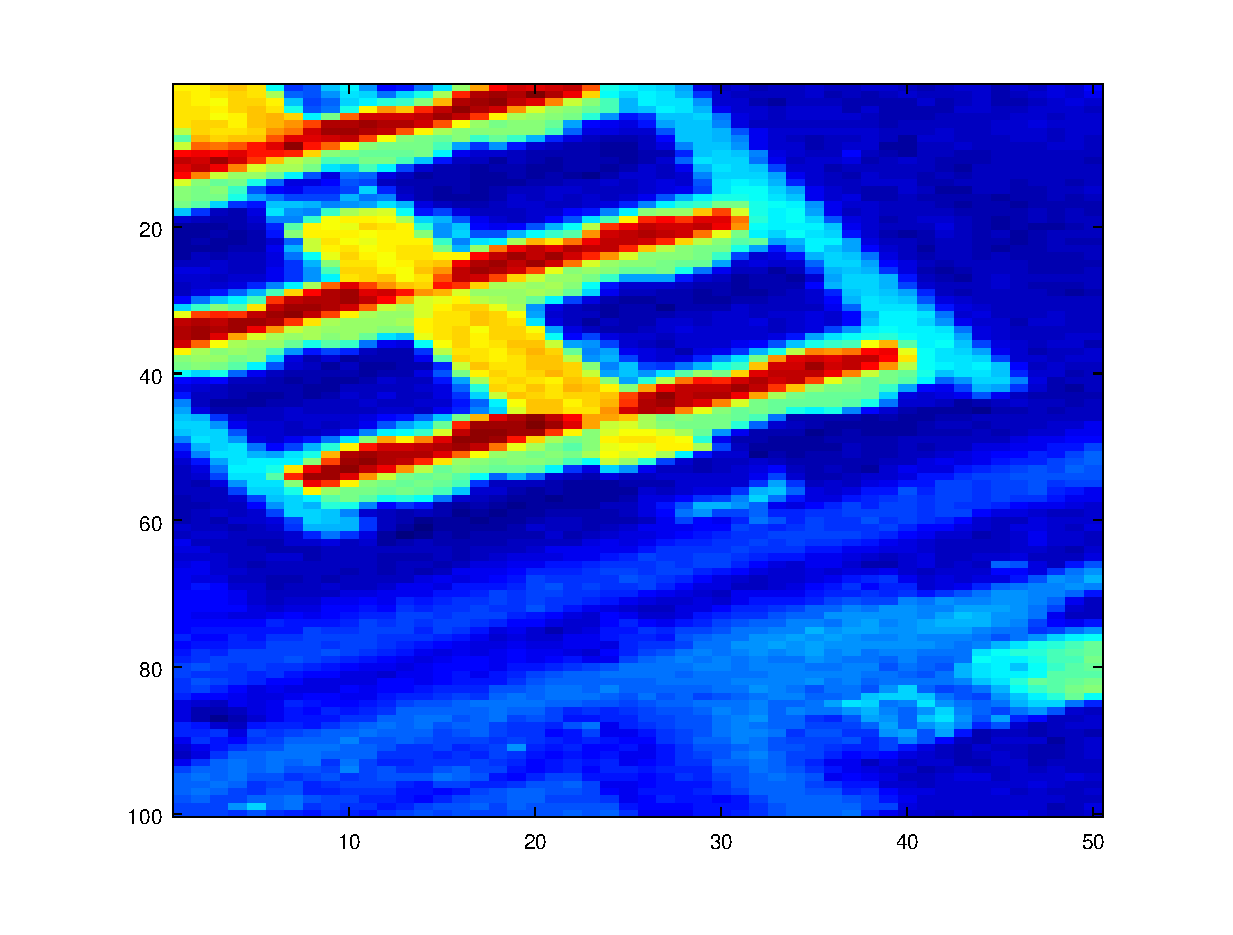
\includegraphics[width=\linewidth]{./Images/paviaSub2/band11.eps}
%   \caption{Low Wavelength}
% \end{minipage}\hfill
% \begin{minipage}{.5\textwidth}
%   \includegraphics[width=\linewidth]{./Images/paviaSub2/myresult.eps}
%   \caption{Spectral Clustering Result}
% \end{minipage}
% \end{figure}
% \begin{figure}
% \begin{minipage}{.5\textwidth}
%   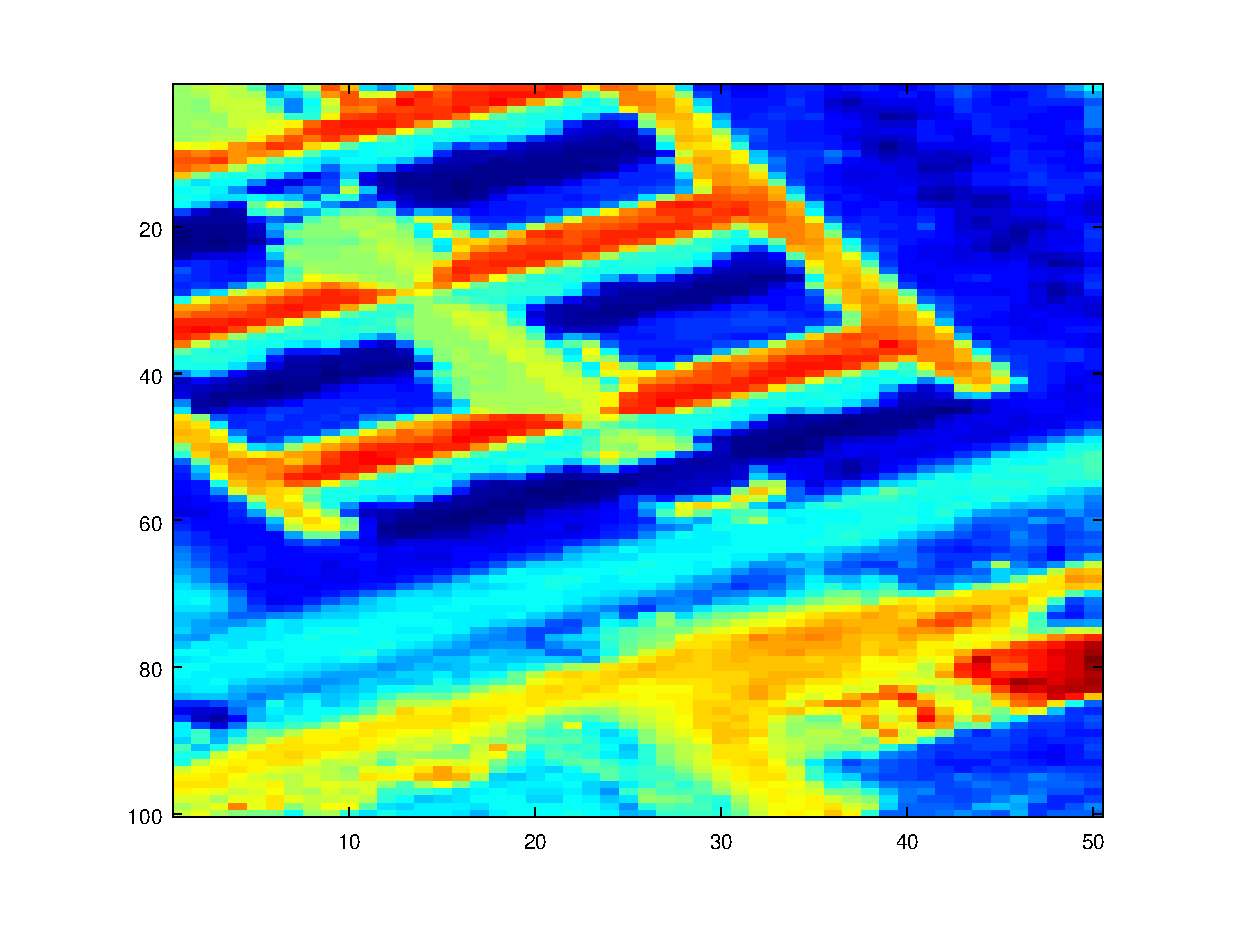
\includegraphics[width=\linewidth]{./Images/paviaSub2/band51.eps}
%   \caption{Mid Wavelength}
% \end{minipage}\hfill
% \begin{minipage}{.5\textwidth}
%   \includegraphics[width=\linewidth]{./Images/paviaSub2/myresult.eps}
%   \caption{Spectral Clustering Result}
% \end{minipage}
% \end{figure}
% \begin{minipage}{.5\textwidth}
%   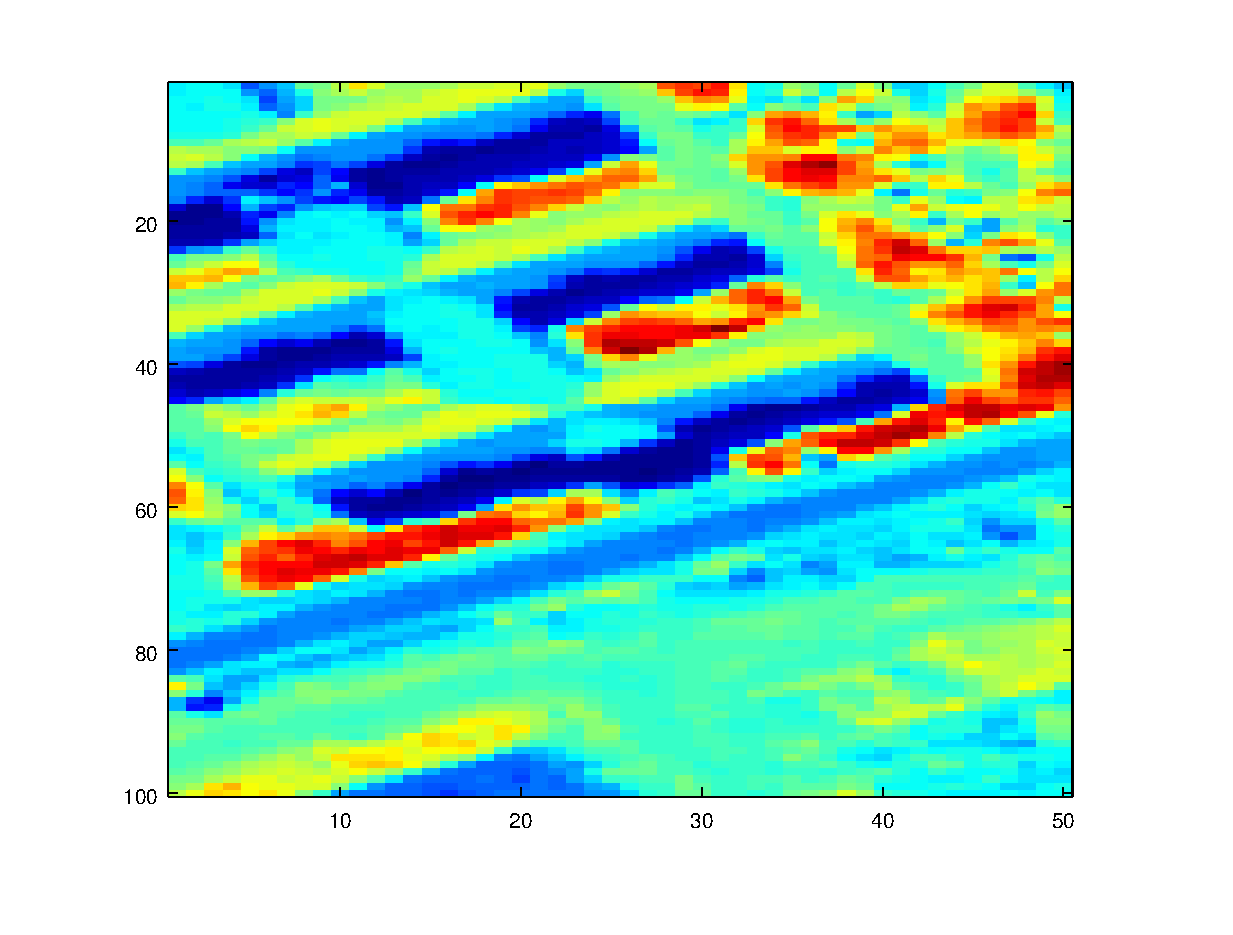
\includegraphics[width=\linewidth]{./Images/paviaSub2/band91.eps}
%   \caption{High Wavelength}
% \end{minipage}\hfill
% \begin{minipage}{.5\textwidth}
%   \includegraphics[width=\linewidth]{./Images/paviaSub2/myresult.eps}
%   \caption{Spectral Clustering Result}
% \end{minipage}
% \end{figure}
% Check against ground truth
% \begin{figure}
% \begin{minipage}{.5\textwidth}
%   \includegraphics[width=\linewidth]{./Images/paviaSub2/myresult.eps}
%   \caption{Spectral Clustering Result}
% \end{minipage}\hfill
% \begin{minipage}{.5\textwidth}
%   \includegraphics[width=\linewidth]{./Images/paviaSub2/groundtruth.eps}
%   \caption{Ground Truth}
% \end{minipage}
% \end{figure}
% \begin{itemize}
% \item Currently, the bottleneck is calculating the Graph Laplacian. Comparing each pair of pixels is too costly.
% \begin{itemize}
% \item Could try subsampling: allow a small number of pixels to represent a larger area.
% \item Could also use Nystr{\"o}m Extension. Eric will talk about this.
% \end{itemize}
% \end{itemize}


\begin{thebibliography}{9}
\bibitem{ref:Pavia}
ROSIS sensor. Hyperspectral image of Pavia University. Data can be obtained at \url{http://www.ehu.eus/ccwintco/index.php?title=Hyperspectral_Remote_Sensing_Scenes\#Pavia_University_scene}

\bibitem{ref:ROSISsensor}
"Hyperspectral Systems, Airborne (ROSIS, HySpex)." Hyperspectral Systems, Airborne (ROSIS, HySpex). N.p., n.d. Web. 09 June 2016.

\bibitem{ref:GraphMinCut}
Goldschmidt, O.; Hochbaum, D. S. (1988), Proc. 29th Ann. IEEE Symp. on Foundations of Comput. Sci., IEEE Computer Society, pp. 444–451

\bibitem{ref:GraphLaplacian1}
Mohar, B. (1991). The Laplacian Spectrum of Graphs. \emph{Graph Theory, Combinatorics, and Applications} Vol 2. pp 871-898. Ed. Y. Alavi, G. Chartrand, O. R. Oellermann, A. J. Schwenk, Wiley.

\bibitem{ref:SpectralClustering1}
Ng, A., Jordan, M., \& Weiss, Y. (2001). On Spectral Clustering: Analysis and an
algorithm. \emph{Advances in Neural Information Processing Systems}, 14.

\bibitem{ref:SpectralClustering2}
Luxburg, U. (2007). A Tutorial on Spectral Clustering. \emph{Statistics and Computing}, 17.

\bibitem{ref:RayleighChebyshev}
C. Anderson, "A Rayleigh-Chebyshev Procedure for Finding the Smallest Eigenvalues and Associated Eigenvectors of Large Sparse Hermitian Matrices", \emph{J. Computational Physics}, vol. 229, pp. 7477-7487, 2010
\end{thebibliography}

\end{document}